\documentclass{standalone}
%\usepackage[dvips]{graphicx}
\usepackage[T1]{fontenc}
\usepackage[active,tightpage]{preview}

\pdfoutput=1
\usepackage[pdftex]{graphicx}

% The figures are in a figures/ subdirectory.
\graphicspath{{../figures/}}

\begin{document}%
\begin{preview}%

\begin{figure}[h]
   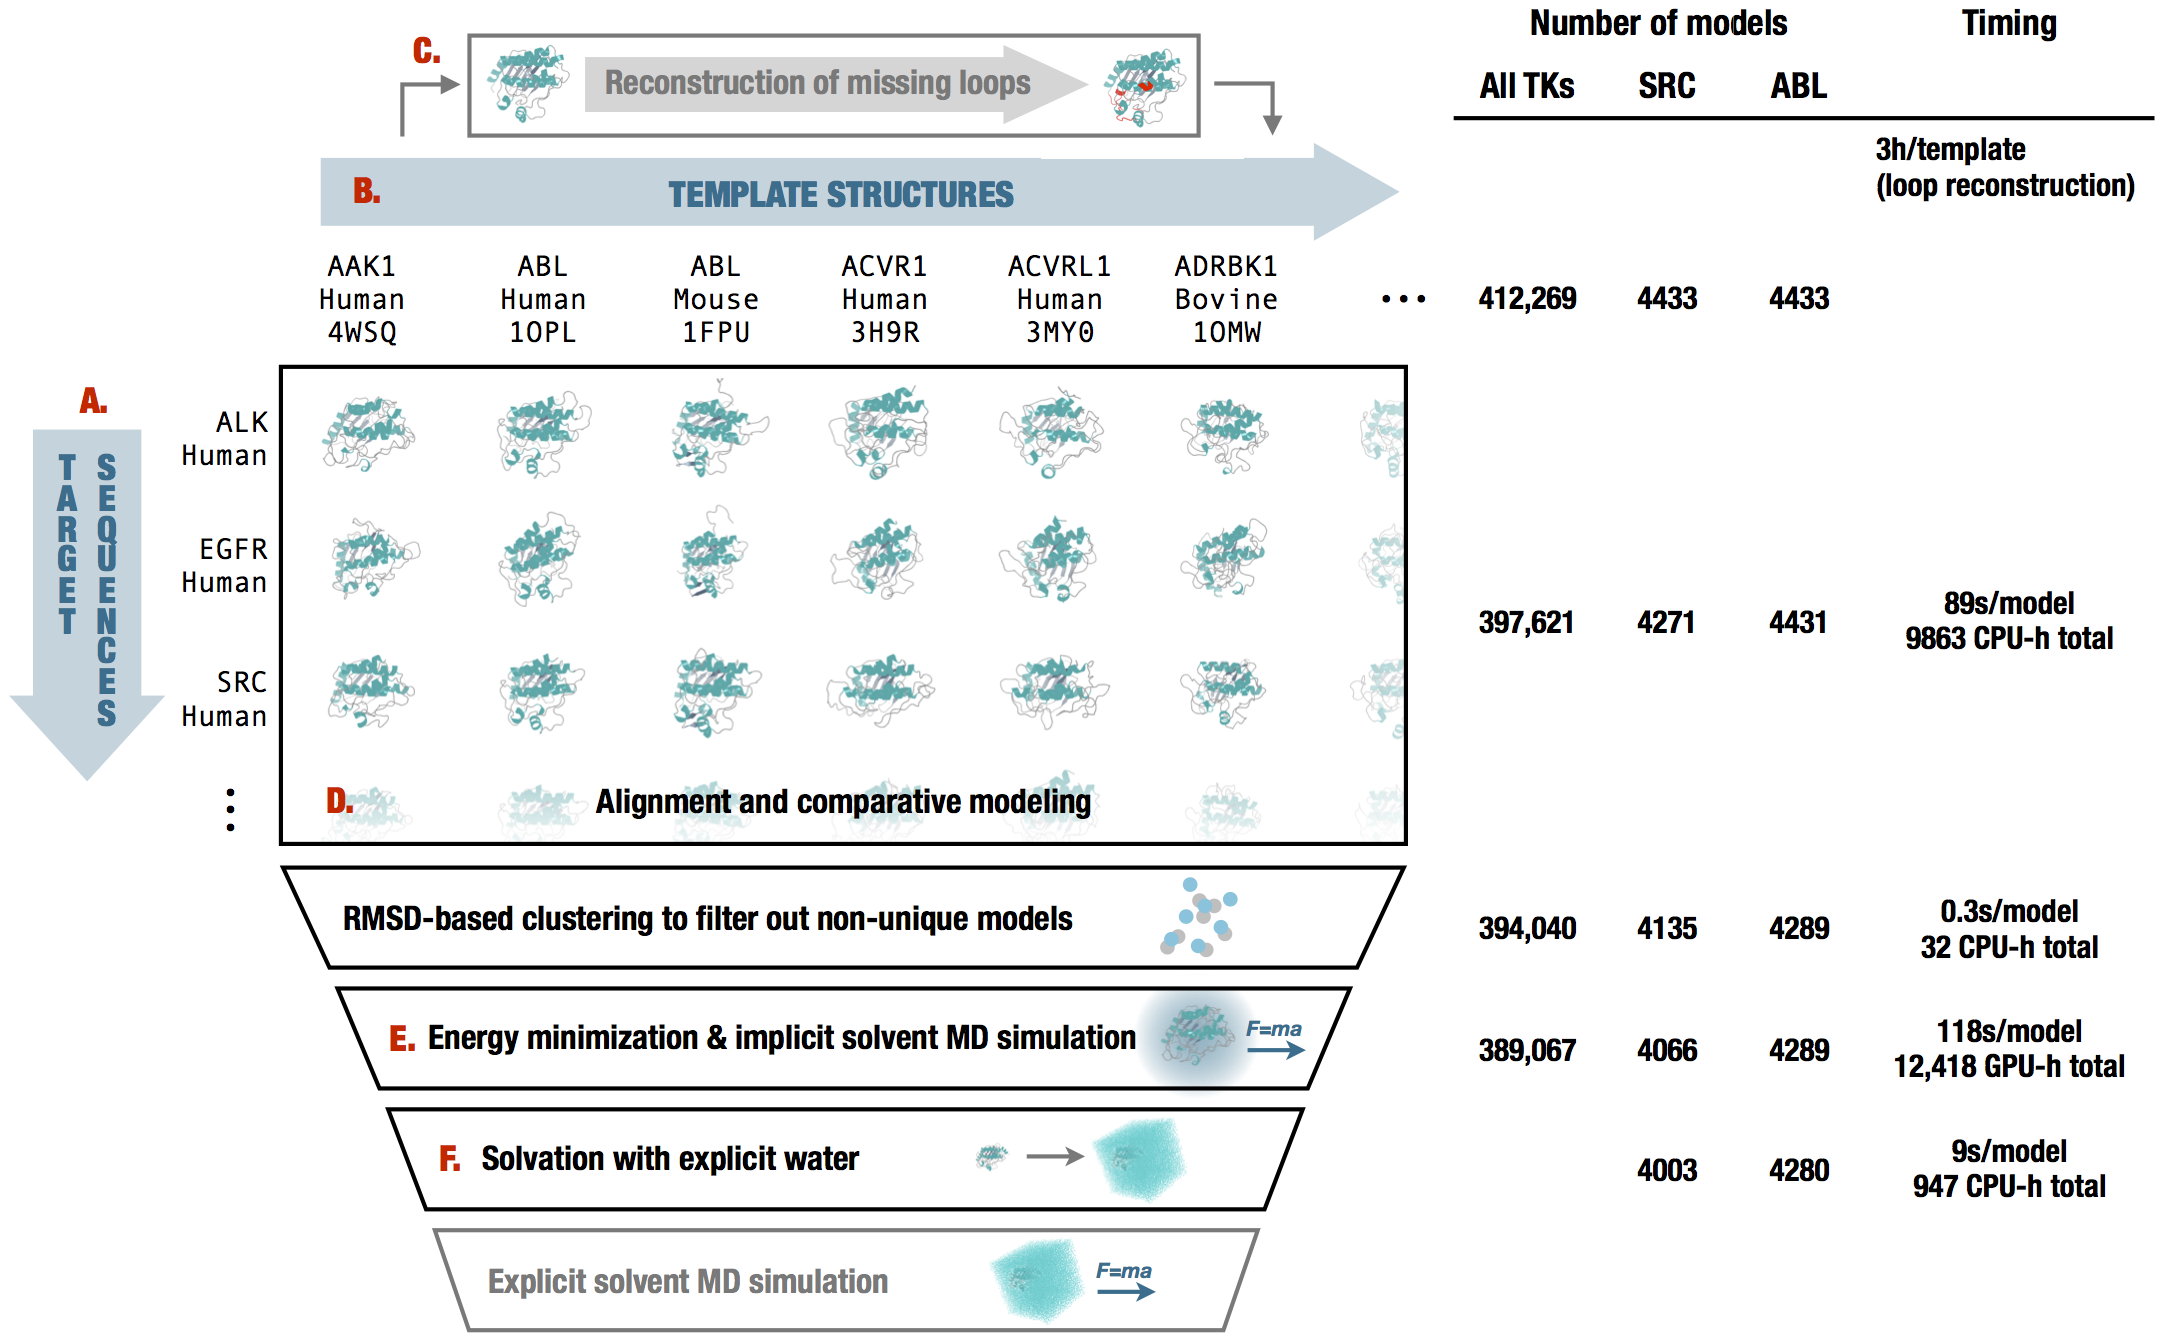
\includegraphics[width=1.0\textwidth]{pipeline/pipeline2}
  \label{figure:pipeline}
\end{figure}

%\begin{figure}[h]
%    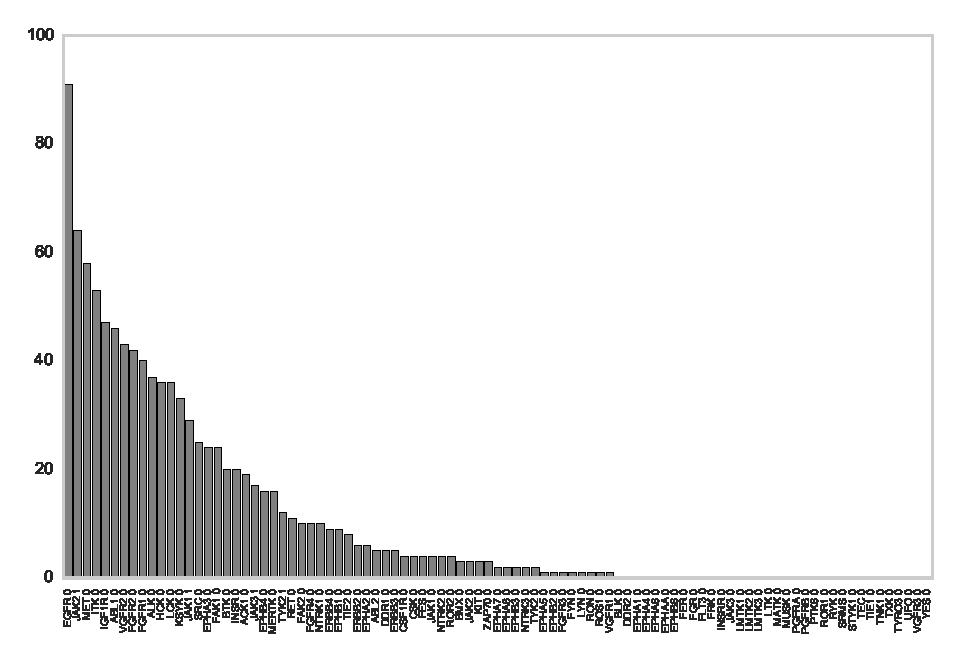
\includegraphics[width=\textwidth]{nstructures_per_tk_target/nstructures_per_tk_target.pdf}
%    \label{figure:nstructures-per-tk-target}
%\end{figure}
%
%\begin{figure}[h]
%    % 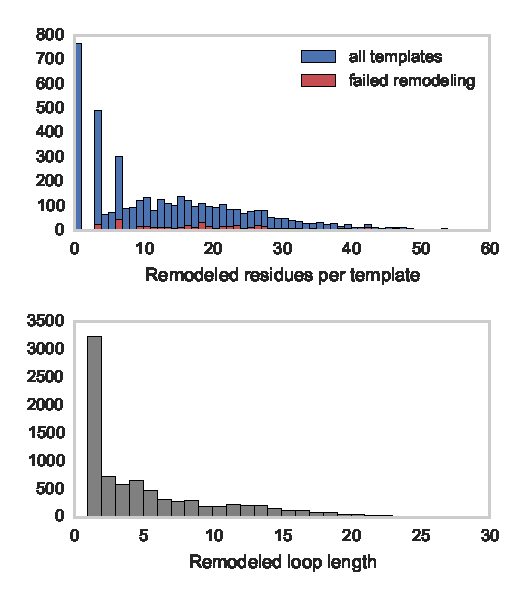
\includegraphics[width=\textwidth]{loopmodel_analysis/nmissing_resis_distributions.pdf}
%    \caption{{\bf Distributions for the number of missing residues in the TK templates.}
%    \emph{Upper:} The number of missing residues per template, for all templates (blue) and for only those templates for which template remodeling with the {\tt loopmodel} subcommand failed (red).
%    Templates for which remodeling failed had a median of 20 missing residues, compared to a median of 14 missing residues for templates for which remodeling was successful.
%    \emph{Lower:} The number of residues in each missing loop, for all templates.    
%}
%    \label{figure:loopmodel-nmissing-residues}
%\end{figure}
%
%\begin{figure}[h]
%    % 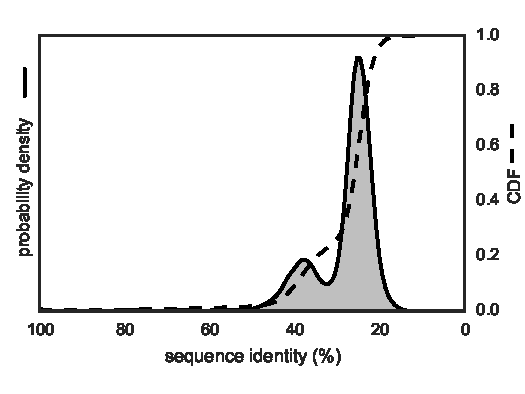
\includegraphics[width=1.0\columnwidth]{seqid_dist/seqid_dist.pdf}
%
%    \caption{{\bf Template-target sequence identity distribution for human tyrosine kinase catalytic domains.}
%    Sequence identities are calculated from all pairwise target-template alignments, where targets are human kinase catalytic domain sequences and templates are all kinase catalytic domains from any organism with structures in the PDB, as described in the text.
%    A kernel density estimate of the target-template sequence identity probability density function is shown as a solid line with shaded region, while the corresponding cumulative distribution function is shown as a dashed line.
%    }
%  \label{figure:sequence-identity-distribution}
%\end{figure}
%
%\begin{figure}[h]
%    % \centering
%    % {\label{figure:rmsd-distribution-joint}%
%    %    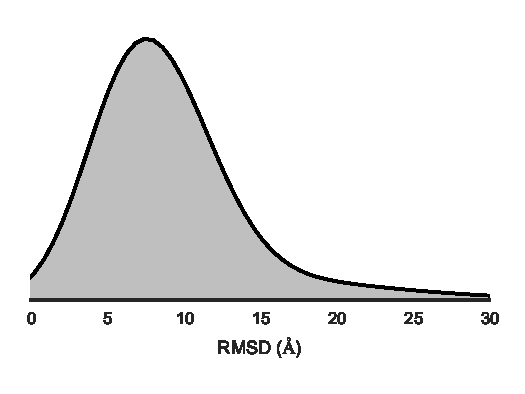
\includegraphics[height=0.6\textwidth]{rmsddist/rmsddist2-joint.pdf}
%    % }
%
%    % {\label{figure:rmsd-distribution-by-sequence-identity}%
%    %    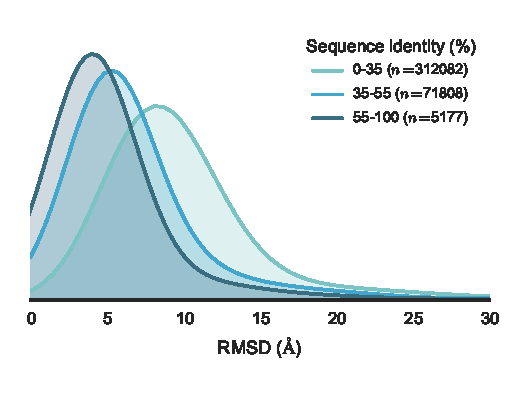
\includegraphics[height=0.6\textwidth]{rmsddist/rmsddist2.pdf}
%    % }
%
%    \caption{{\bf Distribution of RMSDs to all TK catalytic domain models relative to the model derived from the highest sequence identity template.}    
%    Distributions are built from data from all 93 TK domain targets.
%    To better illustrate how conformational similarity depends on sequence identity, the lower plot illustrates the distributions as stratified into three sequence identity classes: high identity (55--100\%), moderate identity (35--55\%), and remote identity (0--35\%).
%    The plotted distributions have been smoothed using kernel density estimation.
%  }
%  \label{figure:rmsd-distributions}
%\end{figure}
%
%\begin{figure}[h]
%    % 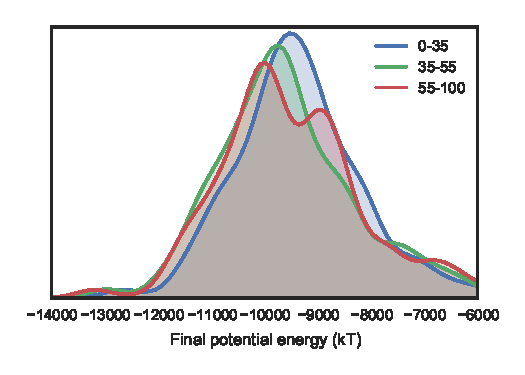
\includegraphics[width=1.0\columnwidth]{energies/energies.pdf}
%
%    \caption{{\bf Distribution of final energies from implicit solvent MD refinement of TK catalytic domain models.}
%    To illustrate how the energies are affected by sequence identity, the models are separated into three sequence identity classes: high identity (55--100\%), moderate identity (35--55\%), and remote identity (0--35\%).
%    The plotted distributions have been smoothed using kernel density estimation.
%    Refinement simulations were carried out at the default temperature of 300~K.
%  }
%  \label{figure:energies-implicit}
%\end{figure}
%
%begin{figure}[h]
%    % 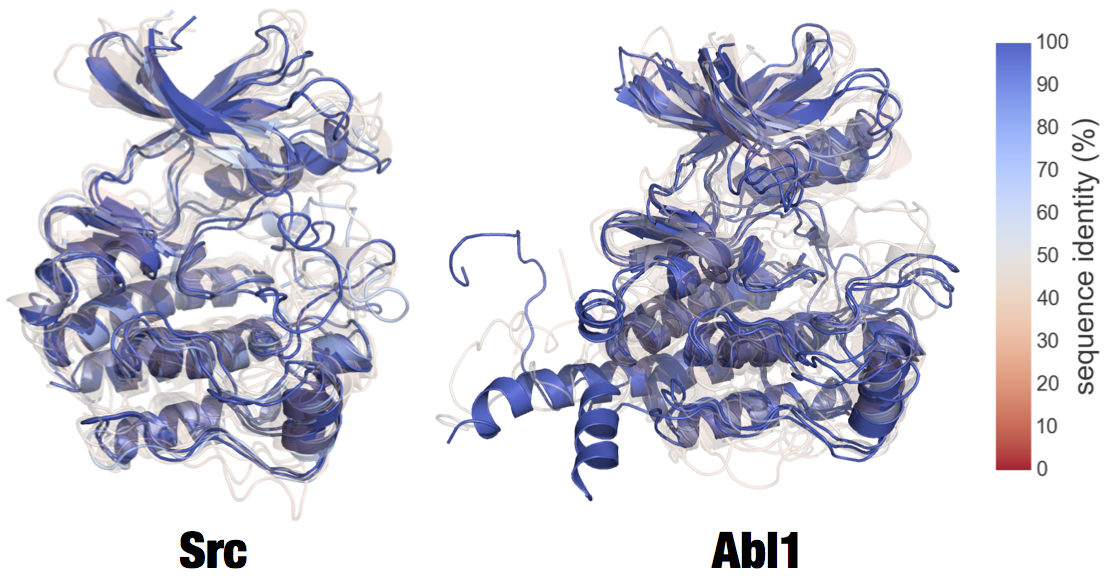
\includegraphics[width=1.0\columnwidth]{superposition-src_abl/superposed-seqid_classes-clustered-one_fig}
%    
%    \caption{{\bf Superposition of clustered models of Src and Abl1.}
%    Superposed renderings of nine models each for Src and Abl1, 
%    giving some indication the diversity of conformations generated by Ensembler.
%    The models for each target were divided into three sequence identity ranges (as in Fig.~\ref{figure:rmsd-distributions}), and RMSD-based $k$-medoids clustering was performed (using the msmbuilder clustering package~\cite{msmbuilder}) to select three clusters from each.
%    The models shown are the centroids of each cluster.
%    Models are colored and given transparency based on their sequence identity, so that high sequence identity models are blue and opaque, while lower sequence identity models are transparent and red.
%  }
%  \label{figure:superposition}
%\end{figure}
%
%\begin{figure}[h]
%    % 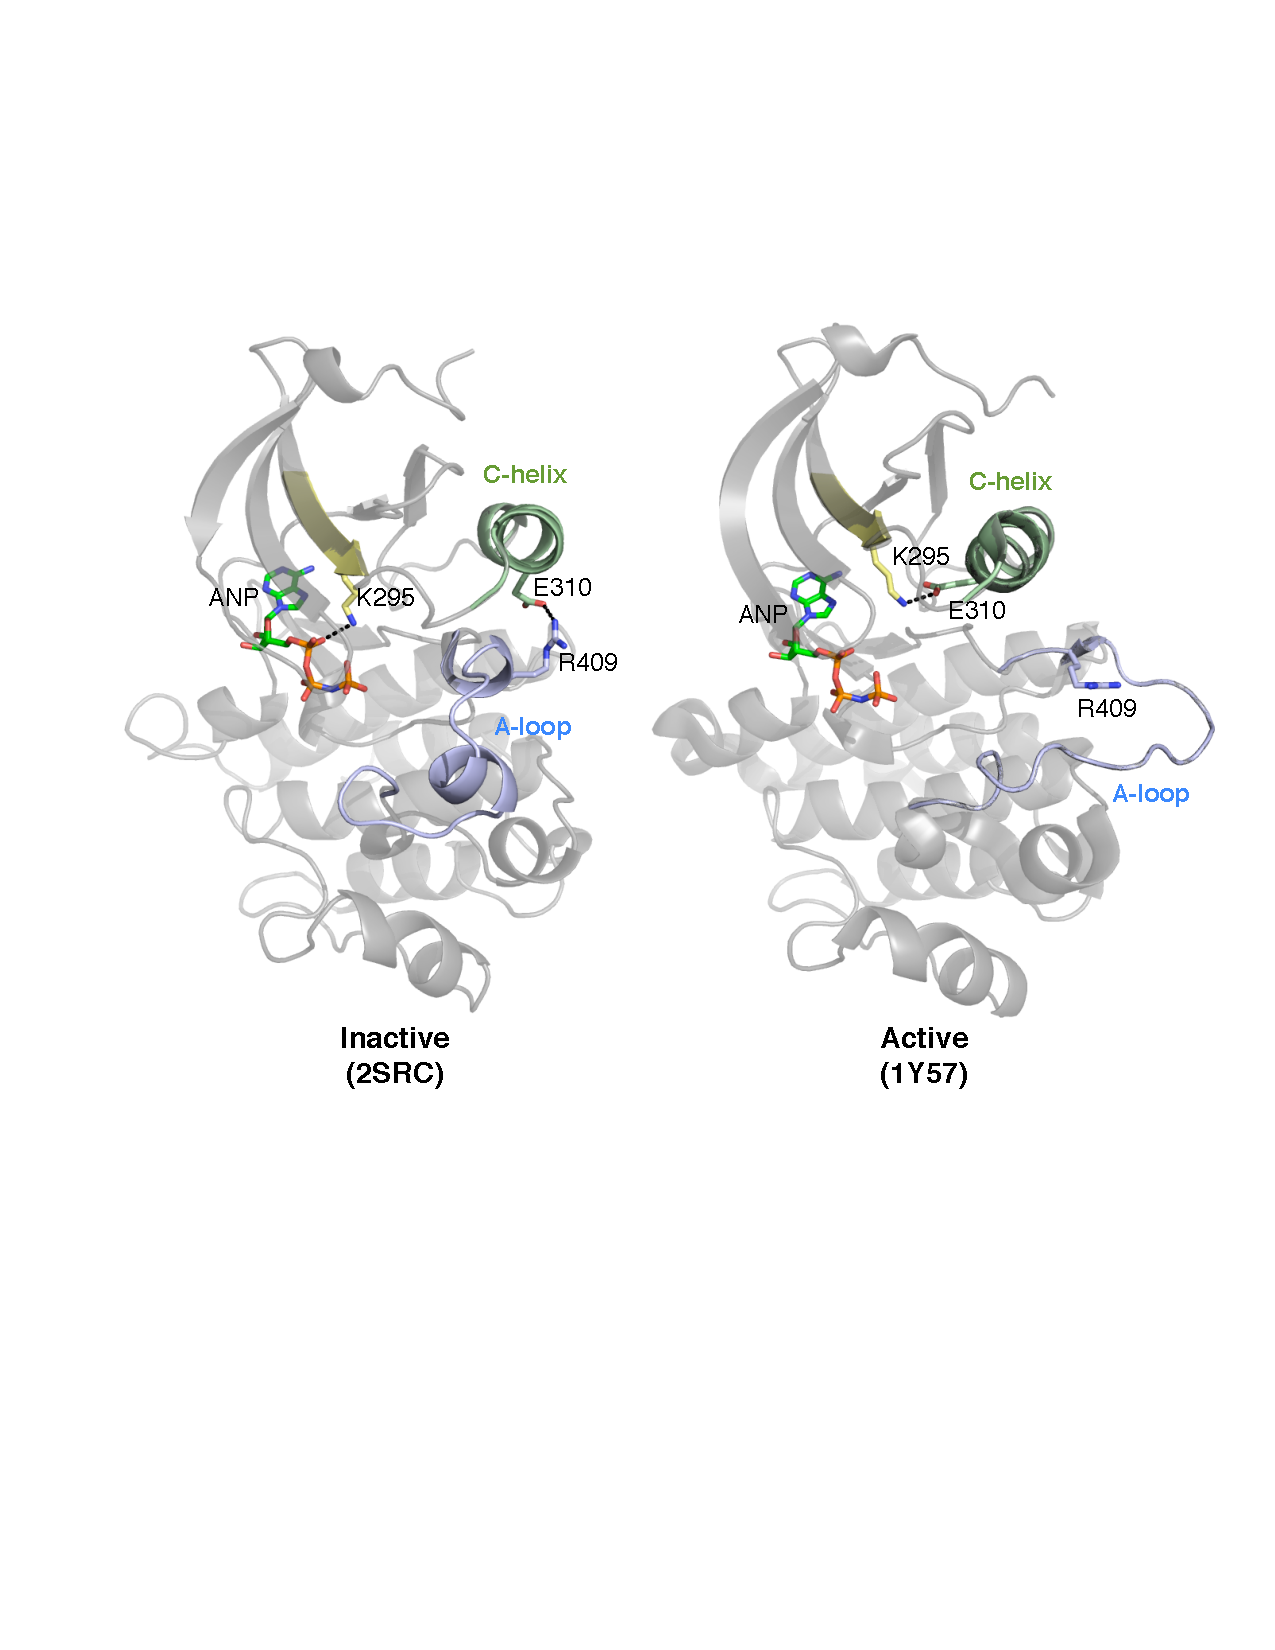
\includegraphics[width=1.0\textwidth]{residue_pair_distances/src/src_ref_structures}
%
%    \caption{{\bf Two structures of Src, indicating certain residues involved in activation.}
%    In the inactive state, E310 forms a salt bridge with R409.
%    During activation, the $\alpha$C-helix (green) moves and rotates, orienting E310 towards the ATP-binding site and allowing it to instead form a salt bridge with K295.
%    This positions K295 in the appropriate position for catalysis.
%    Note that ANP (phosphoaminophosphonic acid-adenylate ester; an analog of ATP) is only physically present in the 2SRC structure.
%    To aid visualization of the active site in 1Y57, it has been included in the rendering by structurally aligning the surrounding homologous protein residues.
%  }
%  \label{figure:src-ref-structures}
%\end{figure}
%
%\begin{figure}[h]
%
%    % \subfloat[Src]{\label{figure:src-distances}%
%    %    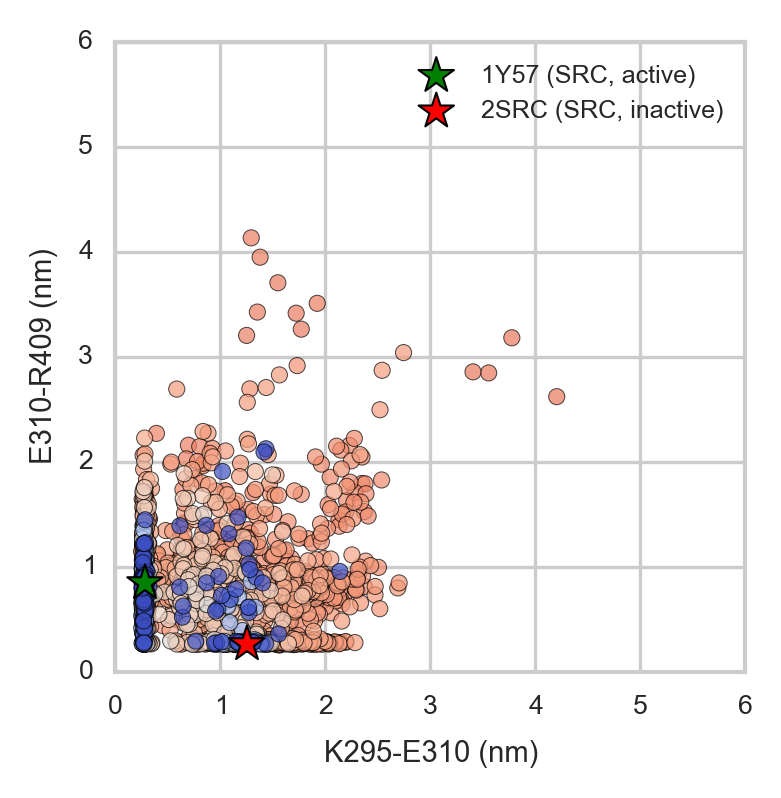
\includegraphics[height=0.31\textwidth]{residue_pair_distances/src_abl_flt4_combined/distances_src.png}
%    % }
%    % \subfloat[Abl]{\label{figure:abl-distances}%
%    %    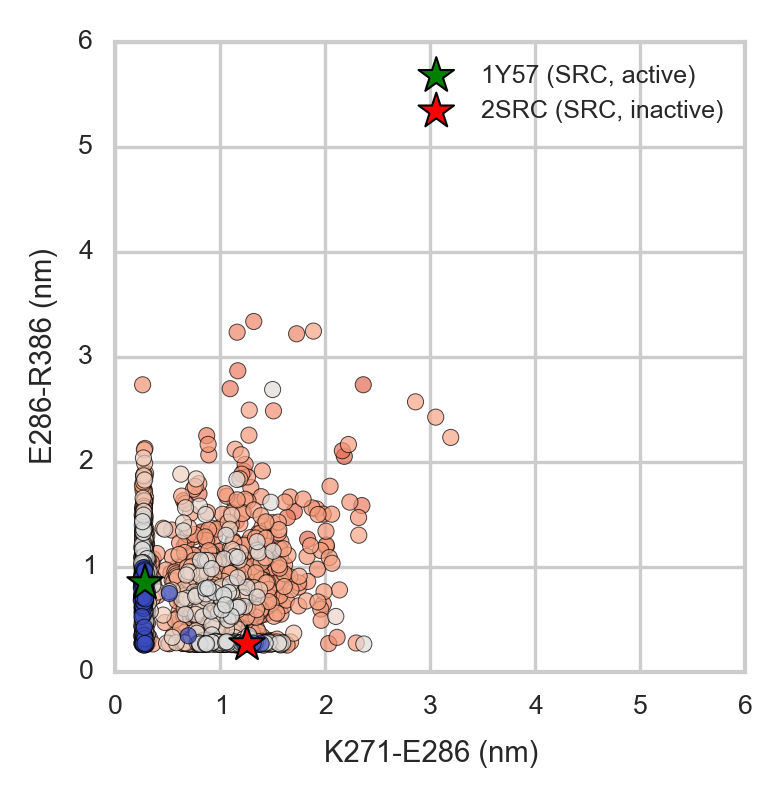
\includegraphics[height=0.31\textwidth]{residue_pair_distances/src_abl_flt4_combined/distances_abl.png}
%    % }
%    % \subfloat[Flt4]{\label{figure:flt4-distances}%
%    %    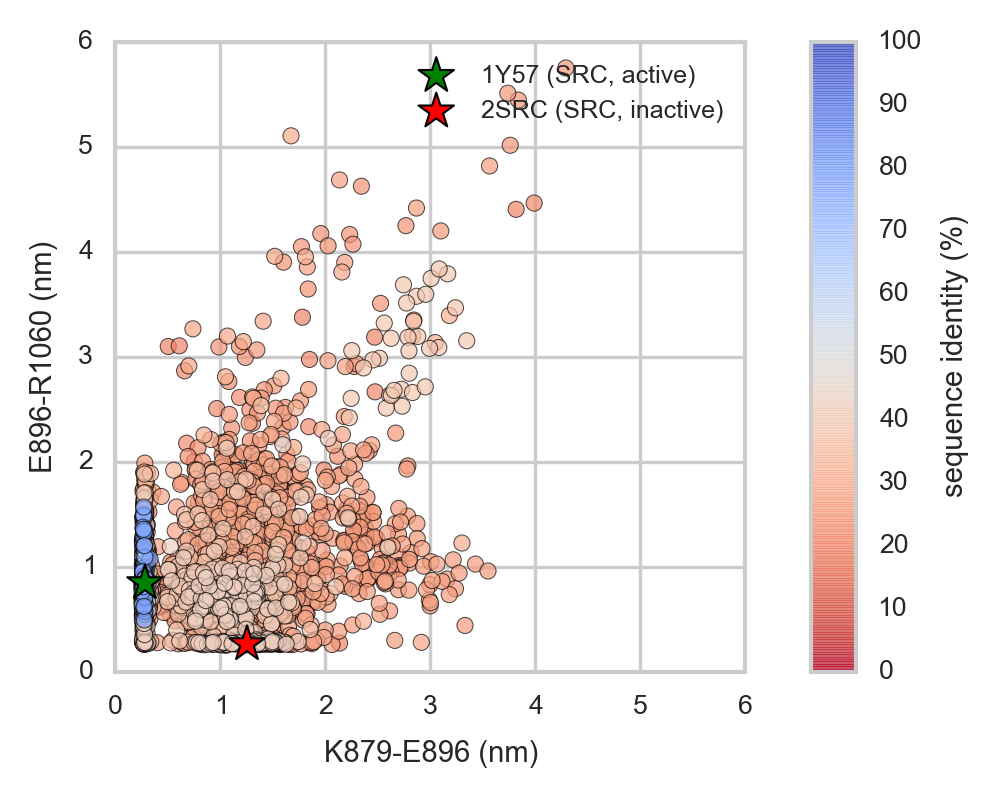
\includegraphics[height=0.31\textwidth]{residue_pair_distances/src_abl_flt4_combined/distances_flt4.png}
%    % }
%
%    \caption{{\bf Src, Abl1, and Flt4 models projected onto the distances between two conserved residue pairs, colored by sequence identity.}
%    Two Src structures (PDB entries 1Y57~\cite{cowan-jacob:2005:1y57} and 2SRC~\cite{xu:1999:2src}) are projected onto the plots for reference, representing active and inactive states respectively.
%    These structures and the residue pairs analyzed here are depicted in Fig.~\ref{figure:src-ref-structures}.
%    Distances are measured between the center of masses of the three terminal sidechain heavy atoms of each residue.
%    The atom names for these atoms, according to the PDB coordinate files for both reference structures, are---Lys: NZ, CD, CE (ethylamine); Glu: OE1, CD, OE2 (carboxylate); Arg: NH1, CZ, NH2 (part of guanidine).
%    }
%  \label{figure:pair-distances}
%\end{figure}

%
%\resizebox{86mm}{!}{%
% put \picture{} here
%}%
%

\end{preview}%
\end{document}
